\documentclass[11pt]{article}
\usepackage{amsmath,amsfonts,latexsym,graphicx}
\usepackage{fullpage,color}
\usepackage{graphicx,wrapfig,ragged2e}

\usepackage{url,hyperref}

% cf https://tex.stackexchange.com/a/325698
\usepackage{etoolbox,setspace}
\AtBeginEnvironment{quote}{\singlespacing\small}

%\pagestyle{empty}

\setlength{\oddsidemargin}{0in}
\setlength{\topmargin}{0in}
\setlength{\textwidth}{6.5in}
\setlength{\textheight}{8.5in}

\newtheorem{fact}{Fact}
\newtheorem{lemma}{Lemma}
\newtheorem{theorem}[lemma]{Theorem}
\newtheorem{defn}[lemma]{Definition}
\newtheorem{assumption}[lemma]{Assumption}
\newtheorem{corollary}[lemma]{Corollary}
\newtheorem{prop}[lemma]{Proposition}
\newtheorem{exercise}[lemma]{Exercise}
\newtheorem{claim}[lemma]{Claim}
\newtheorem{remark}[lemma]{Remark}
\newtheorem{prob}{Problem}
\newtheorem{conjecture}{Conjecture}
\DeclareMathOperator*{\argmax}{arg\,max}

\newenvironment{note}[1]{\medskip\noindent \textbf{#1:}}%
        {\medskip}

\newenvironment{proof}{\vspace{-0.05in}\noindent{\bf Proof:}}%
        {\hspace*{\fill}$\Box$\par}
\newenvironment{proofsketch}{\noindent{\bf Proof Sketch.}}%
        {\hspace*{\fill}$\Box$\par\vspace{4mm}}
\newenvironment{proofof}[1]{\smallskip\noindent{\bf Proof of #1.}}%
        {\hspace*{\fill}$\Box$\par}

\newcommand{\etal}{{\em et al.}\ }
\newcommand{\assign}{\leftarrow}
\newcommand{\eps}{\epsilon}

\newcommand{\opt}{\textrm{\sc OPT}}
\newcommand{\script}[1]{\mathcal{#1}}
\newcommand{\ceil}[1]{\lceil #1 \rceil}
\newcommand{\floor}[1]{\lfloor #1 \rfloor}


\begin{document}

\setlength{\fboxrule}{.5mm}\setlength{\fboxsep}{1.2mm}
\newlength{\boxlength}\setlength{\boxlength}{\textwidth}
\addtolength{\boxlength}{-4mm}
\begin{center}\framebox{\parbox{\boxlength}{\bf
CS 294-149:  \hfill Lecture 4 \hfill Date: 2018-09-04 \\
  Safety and Control for AGI \hfill Scribe: Sam Toyer }}\end{center}

\vspace{5mm}

% \section{Introduction}
%
% We will consider topic X in this lecture.
%
% \begin{theorem}
% This is a result.
% \end{theorem}
% \begin{proof}
% This is the proof.
% \end{proof}
%
% \section{Topic 2}

\section{Introduction}

In the previous lecture, we saw that any agent which satisfies a limited set of
rationality axioms must necessarily have a scalar-valued \textit{utility
function} that fully describes its preference between any pair of ``lotteries''
over future world states.
%
This result is known as the von Neumann-Morgenstern (VNM) utility theorem.
%
Von Neumann and Morgenstern do not require that a rational agent be aware of the
precise utility function that its preferences give rise to, nor require that
artificial rational agents be explicitly constructed as utility-maximisers.
%
Nevertheless, the theorem does suggest that one way to create a rational agent:
specify a fixed utility function describing what we would like the agent to do,
and then program the agent to act in a way which maximises the expectation of
that utility.

\begin{wrapfigure}[23]{R}{0.3\textwidth}
  \vspace{-2em}
  \begin{center}
    
\includegraphics[width=0.2\textwidth]{figures/soviet-nail.jpg}
  \end{center}
  \vspace{-1.5em}
  \caption{
    A Soviet factory manager is awarded a high five for excellence in nail
    production.
    %
    This is how managers were remunerated before the invention of
    rubles.
  }
  \label{fig:nail}
\end{wrapfigure}

Unfortunately, utility-maximisers tend to run afoul of \textit{Goodhart's law},
which anthropologist Marilyn Strathern concisely stated as:
%
\begin{quote}
  When a measure becomes a target, it ceases to be a good measure.
\end{quote}
%
As a example of this, consider the fictitious%
\footnote{
  This fictitious case study started as a parody of the (real) Soviet practice
  of incentivising factory managers based on various measures of gross
  output~\cite{roberts02time}.
}
case
of a factory manager told that they will be rewarded in proportion to the
tonnage of nails produced by their factory.
%
Prior to the introduction of this target, the cumulative mass of produced nails
may have been a reasonable proxy for the total value created by the factory
because all nails were of similar size.
%
However, once the target is in place, the relationship between value and weight
is decoupled.
%
Instead of producing a high volume of small, useful nails, the factory manager
can simply cast a single colossal nail each month with the combined mass of many
millions of small nails (Figure~\ref{fig:nail}).
%
This will likely net the manager a large reward (which may be a bonus, a company
car, or an enthusiastic-but-businesslike high five) at the end of the year.
%
However, it will fail to meet the factory's (presumed) goal of efficiently
creating useful goods.

As AI researchers, we need to be careful to avoid constructing systems that fail
to serve their intended purpose due to Goodhart-type effects.
%
This is a serious risk for expected utility maximisers such as reinforcement
learning agents, which will naturally tend to do some combination of the
following:
%
\begin{enumerate}
  \item Optimise the given utility function \textit{too well} and find
    an unexpected maximum of the utility function that violates the designer's
    intent.
    %
    In contemporary systems this requires further reward engineering on the part
    of the designer to create a utility function that actually reflects their
    desired goal.

  \item Optimise the given utility function \textit{too poorly} and fall into
    a useless local maximum from which the agent cannot escape in a reasonable
    amount of time.
    %
    This is a common problem in applications of reinforcement learning to
    complex systems, which typically requires a carefully shaped reward function
    to help guide the agent's initial exploration towards some useful end.
\end{enumerate}
%
Consequently, researchers and engineers sometimes need to put significant
thought into choosing an appropriate combination of optimiser, transition
dynamics, and reward function that avoids these problems.

In the remainder of these notes, we will see a range of situations where
Goodhart's law, or \textit{reward misspecification}, has cropped up, both in the
real world and in the laboratory.
%
We will also consider alternatives to the specify-and-maximise paradigm of agent
construction that may lead to better-behaved agents.

\section{Categorising instances of Goodhart's law}

One way of understanding Goodhart-type problems is to categorise them according
to their effects.
%
Manheim \& Garrabrant~\cite{manheim18categorizing} present one such taxonomy
targeted towards AI researchers, in which they separate variants of Goodhart's
law into four categories:
%
\begin{description}
  \item[Adversarial]
    Regulator Regina has a goal $G_R$ that she wishes to achieve, and uses a
    proxy utility $U$ to measure how well Adversary Adi is maximising the
    goal.
    %
    Meanwhile Adi has a (possibly incompatible) goal $G_A$, and access to the
    proxy $U$.
    %
    In this situation Adi might choose to modify $G_A$ so that it is correlated
    with $U$---as required by Regina---but without actually maximising $G_R$.

    For instance, Adi might be the nail factory manager from earlier, while
    Regina might be a manager of nail factory managers.
    %
    In this case $G_R$ measures ``productivity'' in some abstract sense, but $U$
    only measures tonnage, so Adi adopts a goal $G_A \approx U$ that allows him
    to collect a large bonus by simply producing a single huge nail.

  \item[Regressional]
    In regressional Goodhart, Regina has a goal $G_R$ that she wishes to achieve
    by directly maximising some proxy measure $U(a) = G_R(a) + N(a)$, where
    $N(a)$ is a noise term.
    %
    If Regina tries to find the optimal action $a = \argmax U(a)$ according to
    $U$, then she will tend to find the one that is highest in \textit{both}
    $G_R(a)$ and $N(a)$.
    %
    In some sense this an unavoidable consequence of maximising \textit{any}
    noisy proxy of a utility function, and is closely related to ``winner's
    curse''---the winning bidder in an auction will tend to be the one who has
    produced the most severe overestimate of the intrinsic worth of an item.

    In an AI context, such a situation may arise from noisy measurements of the real
    world.
    %
    For instance, a UAV might be charged with finding the peak of a mountain
    using noisy measurements from a LIDAR.
    %
    In this case, its highest measurement is likely to correspond to a point
    that is relatively high above the ground but also relatively over-estimated
    due to noise, since $G_R(a)$ (real height of the point) and $N(a)$
    (unavoidable sensor noise) are weighted equally in the utility it is trying
    to maximise.

  \item[Causal]
    Regulator Regina now chooses an objective $U$ which is statistically
    correlated with her true objective $G_R$.
    %
    However, $U$ may not \textit{causally} affect $G_R$ at all, in which case
    optimising $U$ will have no effect on $G_R$.
    %
    There are several further variants of this kind of Goodhart effect that
    capture different kinds of causal independence between $G_R$ and $U$.

    As a simple example, consider ``teaching to the test'': teachers would like
    their students to understand whatever material is being taught at an
    appropriate level.
    %
    However, if a teacher directly improves their students' test-taking ability,
    then they will increase this proxy measure without actually improving the
    students' understanding significantly.
    %
    In other words, test performance is an \textit{indicator} of understanding,
    not a \textit{determinant} of understanding.

  \item[Extremal]
    Finally, Regina may choose a proxy $U$ which \textit{will} lead to an
    increase in $G_R$ if optimised within a typical, reasonable range of $U$s.
    %
    However, at extreme values of $U$---beyond those typically observed in
    practice---$U$ may begin to deviate from $G_R$ in systematic ways, and
    further optimisation of $U$ may make Regina's decisions worse at optimising
    $G_R$.

    As an example, imagine Regina is using logistic regression to classify
    whether a house will meet its reserve price at auction based on certain
    characteristics (e.g. number of bedrooms, floor area, price relative to
    other houses in the postcode, etc.).
    %
    Regina's goal $G_R$ is to maximise the performance on unseen houses that
    might go on the market in the future, but as a proxy $U$ for that
    performance she chooses the algorithm's classification performance on a
    validation set.
    %
    She then chooses a set of hyperparameters (feature space, optimiser, etc.)
    that maximise $U$.
    %
    However, at extremely low levels of validation set error---anything below the
    Bayes error rate, for instance---the relationship between $U$ and $G_R$
    breaks down due to overfitting.
    %
    Hence, Regina may end up choosing a complex set of hyperparameters that
    produce a model which has zero validation error, but which fails to
    generalise well.
\end{description}


\section{Goodhart's law in action}

\subsection{Examples from human society}

The effects of Goodhart's law can be observed in a wide variety of human social
structures.
%
In 1975, Kerr~\cite{kerr75folly} collected a number of these examples, and put
them in a paper targeted at managers with the tagline ``it's the reward system,
stupid!''
%
Examples from Kerr's paper and elsewhere include:
%
\begin{enumerate}
  \item Professorial teaching incentives: university departments would like their
    academic staff to offer high-quality courses, but many departments choose to
    reward research output to the exclusion of teaching achievements.
    %
    Hence, professors choose to allocate more of their time to research than
    teaching, and teaching quality suffers as a result.

  \item Corporate whistleblower incentives: the US Securities and
    Exchange Commission (SEC) rewards third-party whistleblowers who inform them
    of large corporate frauds to up to 30\% of the total amount of money
    involved in the fraud.
    %
    Unfortunately, this encourages potential whistleblowers to indirectly
    perpetuate and ``run up the total'' of a fraud as much as they can in order
    to get a larger payout.

  \item Rats' tails: Vann~\cite{vann03rats} notes that French colonial officers
    in Vietnam once instituted a scheme in which locals would be paid for each
    rat's tail delivered to a local colonial bureaucrat.
    %
    The aim of this scheme was to reward people for killing rats, using tails as
    a convenient form of evidence.
    %
    Unfortunately, this gave rise to a new class of tail collectors who would
    simply cut the tails off captured rats.
    %
    They would then re-release the rats so that they could procreate and produce
    further rats for ``harvest''.
\end{enumerate}

These sorts of flawed incentive systems do not necessarily arise from
incompetence on the part of incentive-setters.
%
One particularly powerful force towards broken incentive systems is the desire
for transparent, objectively measurable targets.
%
The number of citations received by a professor, the amount of money involved in
a fraud (as measured by the SEC), and the number of rat tails delivered to a
French bureaucrat are all reasonably objective and easy-to-measure quantities.
%
However, they can easily decouple from the true (possibly subjective) goal for
the relevant system.
%
Unfortunately, any target we give an AI system \textit{must} be objective in
order for us to implement it, so as AI researchers we can only ameliorate---and
not escape---this source of Goodhart-type scenarios.

\subsection{Examples from genetic programming and artificial life}

In addition to human social structures, Goodhart's law also asserts itself in
artificial intelligence research.
%
Lehman~\etal\cite{lehman18surprising} document dozens of instances of
experiments in genetic programming and artificial life that yielded surprising
and unintended consequences due to a combination of reward misspecfication,
simulator flaws, and the intrinsic ``creativity'' of random search.
%
They organise their examples into four broad themes---\textit{selection gone
wild}, \textit{unintended debugging}, \textit{exceeding expectations}, and
\textit{convergence with biology}---that are described in further detail below.

\begin{figure}
  \begin{center}
    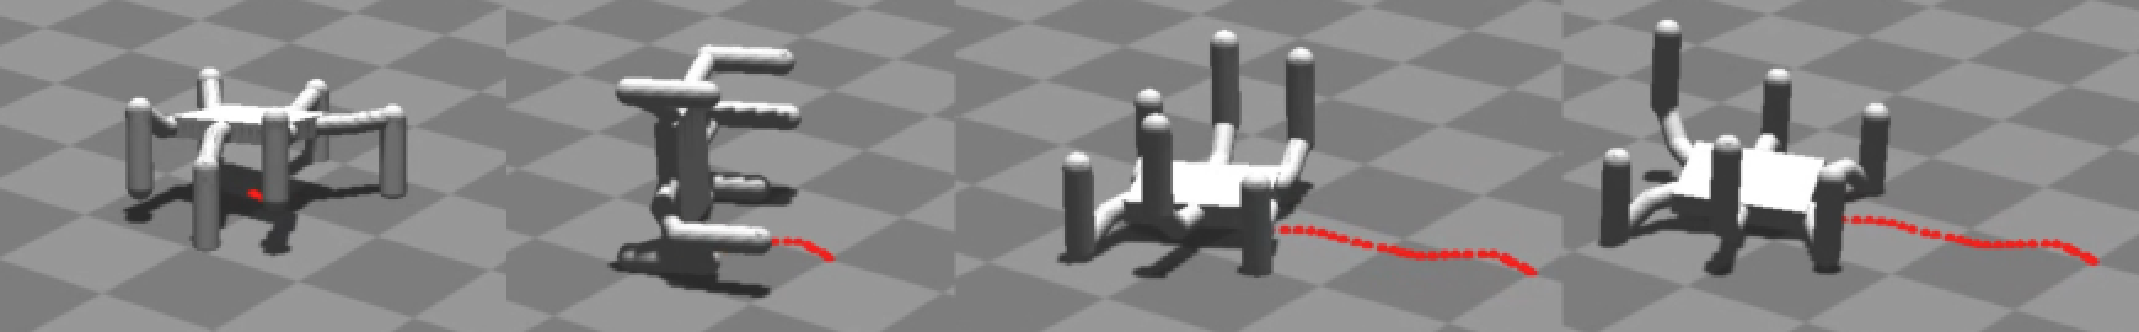
\includegraphics[width=0.95\textwidth]{figures/elbow-walking-robot.png}
  \end{center}
  \vspace{-1em}
  \caption{
    This example from Lehman~\etal\cite{lehman18surprising} shows a creature
    that learnt to ``walk'' on its elbows after being tasked with learning a
    walking gait which did not require its feet to touch the ground.
  }
  \label{fig:elbows}
\end{figure}

\paragraph{Selection gone wild}
%
Lehman~\etal note that ``digital evolution [sometimes] reveals the divergence
between what an experimenter is asking of evolution and what they \textit{think}
they are asking''.
%
In particular, ``experimenters often overestimate how accurately their
quantitative measure reflects the underlying qualitative success they have in
mind'', and it is ``often functionally simpler for evolution to exploit
loopholes in the quantitative measure than it is to achieve the actual desired
outcome''.
%
This is essentially a restatement of Goodhart's law as it applies to AI, and the
related anecdotes have a similar flavour to those collected by
Kerr~\cite{kerr75folly}.

One example is that of an artificial creature that was evolved to high-jump.
%
As a proxy measure for this ability, the researchers measured the maximum height
above the ground of the creature's centre-of-mass.
%
However, this lead to creatures with stout bodies atop long, thin legs.
%
Hence, the researchers iterated and used a different proxy reward: the peak
height of the part of the creature that was originally closest to the ground.
%
Unfortunately, this led to a similar class of creatures that would kick off from
the ground using a tall appendage in order to somersault, thus placing the
previous lowest part of the creature high into the air!
%
This and related examples are well worth reading to see how Goodhart's law can
rear its head in real AI research.

\paragraph{Unintended debugging}
%
Optimising some simple quantity in a simulated environment can sometimes reveal
bugs in the simulation itself.
%
One striking example was the discovery, due to a genetic programming algorithm,
of a previously-unknown bug in the Atari game Q*bert.
%
The algorithm discovered a particular sequence of actions which allowed the
player character to destroy an enemy in a way that would normally kill the
player character as well.
%
However, due to a bug in the game, the player character's death was not
penalised, and the algorithm was able to repeat the relevant sequence of actions
until the game score rolled over.
%
This class of anecdotes demonstrates that RL-type algorithms are not only
dependent on a well-specified reward, but also on environment models that remain
accurate even when simulating unusual action sequences.

\paragraph{Exceeding expectations}
%
Sometimes expected utility maximisers discover useful or interesting ways of
maximising utility that the experimenters did not foresee.
%
In contrast to the previous two classes of anecdotes, examples from this class
often show the \textit{desirable} effects of maximising a well-chosen utility
defined in an accurately simulated environment.

Figure~\ref{fig:elbows} shows one example of ``exceeded expectations'': some
roboticists wished to test how robust an evolutionary control algorithm was to
failures in the appendages of a legged robot.
%
They evaluated how well the algorithm could make the robot move forward with
different fractions of its feet touching the ground.
%
With none of the feet enabled, the researchers expected the robot would not be
able to move forward at all.
%
Instead, they found their control algorithm was robust enough to learn how to
flip the robot onto its back and walk with its elbows.

Another example comes from the evolution of control strategies for Braitenberg
vehicles.
%
These are simple circular robots with two drive wheels and a light sensor that
must drive towards a light source in the environment.
%
Typical human-coded control strategies force the vehicle to keep the light
source straight ahead of it by alternately moving forward with one wheel and
then the other.
%
However, genetic programming discovered a strategy that involved repeatedly
spinning around while varying the speeds of wheels during the spin to ensure
forward progress.
%
This unconventional strategy was found to be \textit{more} effective than
typical human-coded strategies at high speeds, since the traditional control
strategy struggles to respond quickly enough to rapid changes in light position.

\paragraph{Convergence with biology}
%
Occasionally the use of evolutionary algorithms gives rise to structures that
parallel those found in real, naturally-evolved organisms.
%
Lehman~\etal included examples of simulated soft-body creatures that evolved
leg-like appendages and learnt gaits reminiscent of those found in animals.
%
Examples in this category are an interesting validation of the ability of
``artificial life'' techniques to recreate behaviours seen in the real world,
but are less relevant to our concerns in this course.

\paragraph{More examples}
%
The examples above are mostly taken from artificial life and genetic programming
researchers.
%
Victoria Krakovna and others have also curated a broader collection of examples
of AI systems ``gaming'' their specified reward functions which includes
examples from outside that
community.\footnote{
  \url{https://vkrakovna.wordpress.com/2018/04/02/specification-gaming-examples-in-ai/}
}%
\footnote{
  In a comment on Victoria's blog post, Stuart Russell points out that
  ``gaming'' and ``reward hacking'' misleadingly imply that misaligned agent
  know the values they ought to maximise, but choose not to maximise those values.
  %
  The term ``misspecification'' is used throughout most of these notes to
  reflect the fact that misalignment is more likely to arise from inadequate
  system design than from actual malice on the part of the agent itself.
}
%
Notable recent entries on the list include the Q*bert bug mentioned above, and
the CoastRunners reward misspecification flaw that Anca referred to last
week.\footnote{\url{https://blog.openai.com/faulty-reward-functions/}}

\section{Overcoming Goodhart}

% Things to talk about:
%
% - Include the `components of the RL problem' slide from earlier. I think the
%   decomposition there is really important (do problems arise from the
%   optimiser? The transition model? The reward?).
% - Point out that Dan's example suggests we should not 
% - Use example of self-driving car to drive discussion of fixing the
%   \textit{reward}.
% - Philosophical problem with weighting contributions from different utility
%   functions.
% - Alternatives to RL with possibly-faulty reward:
%    * Treat rewards as latent variable that you do IRL to recover.
%      ---> Use `invert a neural net!' as example of what may go on when you try
%           to optimise against a learnt reward function. V hard to do unless
%           you have some way of maximising the reward *while keeping things on
%           manifold of reasonable trajectories*.
%      ---> Ties into concern about uncertainty in IRL; RL is bad at 'knowing
%           what it knows' & tends to do stupid things due to overconfidence.
%    * Quantilisers, that take known distribution over outcomes & try to get
%      outcome in top X% rather than outcome at the very top.
%    * Hard constraints on not doing stupid shit.

\subsection{Fixing specification defects by not using defective specifications}

\begin{quote}
  \begin{flushright}
  If you're having misspecfication problems I feel bad for you, son.\\
  %
  I got 99 problems and my robot's utility function accounts for every one.\\
  \vspace{0.5em}
    {\sc --- Jay-Z} (probably)
  \end{flushright}
\end{quote}

Goodhart-type effects are undesirable because the violate preferences of the
system designer that the designer did not think to put into the system's utility
function, or which they could not find a practical way to put into the system's
utility function.
%
Some of those hidden utilities might include the value we place on liberty,
fraternity, and equality, or other things that we either take for granted until
they are absent or which we cannot directly force a system preserve.
%
However, if we can systematically enumerate and codify \textit{all} (or most) of
those values then we may end up with a utility function that is less vulnerable
to Goodhart-type effects.

As a class, we have been through this exercise twice with self-driving
cars---what sort of utility function would a owner of a self-driving car want
their car to maximise?
%
Some of the preferences suggested by students include
%
\begin{itemize}
\item minimising time to destination,
\item not crashing,
\item ensuring a smooth ride,
\item maximising fuel efficiency,
\item being courteous to other road users,
\item maximising star rating for the car on Yelp or similar,
\item and so on.
\end{itemize}
%
This list is not complete, but does hint at some of the challenges in defining a
``complete'' reward function.
%
Some criteria are well-defined and relatively easy to optimise directly (eg
minimising time to destination), but only cover a small fraction of what we'd
like the car to do.
%
Others encompass more of our values (eg maximising star rating), but are much
harder to measure or maximise efficiently.
%
The challenges associated with creating specifications for more complex systems
are even more severe.

\subsection{Treating reward as a latent variable}

% Things to mention:
% - IRL and (flawed) assumption of demonstrator rationality
% - `AI is pretty bad about knowing what it knows' & so struggles to act
%    conservatively
% - Taking about distributions over utility functions at all is possibly a bad
%   idea because VNM-style utility functions can't be directly compared to one
%   another. Use example from class and link it back to social choice
%   theory/interpersonal utility functions.

An alternative approach to avoiding Goodhart-type problems is to introduce
uncertainty over the true reward function, and have the agent treat the true
reward as a latent variable that must be recovered through exploration.
%
Inverse Reinforcement Learning (IRL) is one popular way of doing just
that~\cite{ng00algorithms}.
%
In IRL, an agent is given a set of demonstrations produced by an
expert---probably a human---and must recover the reward function that the
demonstrator was maximising.
%
Because the basic IRL problem is typically extremely under-constrained, it is
necessary to make strong assumptions about the demonstrator themselves.
%
In particular, most IRL algorithms assume that the demonstrator is an optimal or
near-optimal actor---for instance, that the log probability $\log p(\tau)$ of a
trajectory $\tau$ is proportional to the cumulative reward $R_\tau$ of the
trajectory.
%
This ensures that that any trajectory $\tau$ with very low return $R_\tau$ is
unlikely to occur in the demonstration set.
%
Unfortunately such assumptions are generally not true of humans, who can deviate
from optimal maximisation of their purported utility functions in complex,
time-dependent ways.

Techniques that treat reward as a latent variable also run into all of the
problems related to interpersonal utility comparison.
%
Although the VNM theorem tells us that we can express a single agent's
preferences over all possible world states using a scalar-valued utility
function, it makes no guarantees about the comparability of utility functions
for agents with \textit{different} preferences; maximising a weighted
combination of utility functions is not guaranteed to produce an outcome that is
fair or otherwise desirable.
%
Utility monsters are one example of this: if one agent places very high utility
on a particular outcome $o \in \mathcal O$ and zero utility on any other outcome
$o' \neq o \in \mathcal O$, then that agent's utility can easily outweigh the
utilities of agents that place intermediate (but possibly distinct) utilities on
all $o \in \mathcal O$.
%
Whenever you take an expectation with respect to a distribution over utility
functions, you are necessarily calculating a weighted combination of different
and possibly incompatible utilities and thus making your result vulnerable to
these kinds of failures.

\subsection{Bounded optimisation}

% Talk about quantilisation and Dan's ideas here. Remember to link to that MIRI
% paper to support discussion (Quantilizers: A Safer Alternative to Maximizers
% for Limited Optimization).

Goodhart's law can arise when a system applies ``extreme'' optimisation pressure
to an objective that does not perfectly capture the system designer's desires.
%
If the optimiser is less proficient then Goodhart-type effects may be less
prevalent.
%
Quantilisation~\cite{taylor16quantilizers} is one proposal for such a bounded
optimisation process.
%
Rather than attempting to maximise the expectation of a utility function, a
quantiliser instead takes a distribution over utilities and attempts to produce
an outcome for which the utility merely lies in the top $x\%$ of that
distribution.
%
In other words, a quantiliser aims for an outcome that's ``good enough'' instead
of an \textit{optimal} outcome.

\subsection{Hard constraints and safeguards}

If we can precisely specify the sort of behaviours we would \textit{not} like an
agent to engage in---or, equivalently, to whitelist those behaviours which we
consider safe---then we might be able to make an AI system safe by forbidding it
from engaging in those behaviours.
%
The field of ``safe RL'' has considered a range of approaches along these
lines~\cite{garcia15comprehensive}, including: using a ``shield'' that can
blacklist certain actions where they might be unsafe; creating algorithms that
directly constrain the probability of ending up in certain unsafe states; or
adding a soft requirement that the agent only visit parts of state space that
allow it to eventually return to the initial state.
%
Enforcing such constraints in the absence of an accurate world model is
intrinsically difficult, however.
%
Further, including hard constraints and safeguards can prevent certain problems
at the cost of introducing others; specifically:
%
\begin{description}
  \item[Guardrail effects]
    Sometimes the limitations of a safety guard are poorly understood by human
    decision-makers, which leads to a higher incidence of risky behaviour and
    consequently a greater frequency of undesirable events.
    %
    This effect is named for highway guardrails, which are reputed to sometimes
    \textit{increase} the frequency of vehicle accidents by encouraging
    complacence by drivers.
    %
    In an AI context, we could similarly see human decision-makers choosing to
    deploy a poorly-designed and under-tested AI system because it ``has
    safeguards'', not realising that those safeguards are not insufficient to
    prevent all undesirable incidents.
    %
    Safe-driving cars---which have so far seen wide testing on public roads
    despite significant, and occasionally fatal, software deficiencies---are
    arguably a present-day example of this.

    % Arguably, this has already happened to self-driving cars built by Tesla and
    % Uber, whose systems have been involved in at least three known fatalities
    % (as of mid-2018).
    % %
    % In all three cases, drivers appear to have placed an undue degree of trust
    % in the autonomous (or partly-autonomous) systems, possibly based on
    % experience with the systems' safeguards operating correctly in the past.

  \item[Failed-levee effects]
    Instituting safeguards can also lead to behavioural changes in the people
    and systems that interact with those safeguards, potentially increasing the
    probability of catastrophic failures when the safeguards' limits are exceeded.
    %
    This effect is named for flood levees, which drive down the frequency of
    typical (often small) floods, but which have limited capacity to prevent
    large floods (and can even worsen their effects).
    %
    Reduced flood frequency encourages people to build homes and businesses in
    the previously-unoccupied area downstream of a levee, which may be
    subsequently destroyed in the event of a very large flood.
    %
    In this way, the damage wrought by rare events can be even more disastrous
    than it would be had the levee (or other safeguard) never been constructed.
    %
    Again, in an AI context we might have a learning agent trained with
    safeguards that rarely fail (or constraints that are rarely violated) might
    adopt reckless behaviour that relies on those safeguards consistently
    protecting it.
    %
    This could in turn lead to a higher probability of actions that turn out to
    be extremely dangerous in those rare states where the safeguards fail.

    % This is not a purely sociological phenomenon.
    % %
    % We can imagine that a bipedal industrial robot that is tethered to the roof
    % of a warehouse to prevent it from falling may learn to treat the safety
    % tether as though it were designed to regularly bear loads.
    % %
    % If an excessive load was placed on the tether---for instance, if the robot
    % used it to anchor itself while lifting a heavy object---then the resulting
    % collapse may be even more damaging than a ``typical'' collapse without the
    % safety tether.
    % %
    % The problem is not merely that the safeguard failed, but that the safeguard
    % modified the behaviour of the agent so that the distribution over failure
    % cases was skewed towards rare-but-spectacular disasters.
\end{description}

\bibliographystyle{plain}
%% To add references, uncomment the following two lines and
%% add the relevant bibitems.

\begin{thebibliography}{99}
\bibitem{garcia15comprehensive}
Garcıa, Javier, and Fernando Fernández. ``A comprehensive survey on safe
reinforcement learning.'' \textit{JMLR} 16.1 (2015): 1437-1480.

\bibitem{kerr75folly}
Kerr, Steven. ``On the folly of rewarding A, while hoping for B.''
\textit{Academy of Management journal} 18.4 (1975): 769-783.

\bibitem{lehman18surprising}
Lehman, Joel, \etal ``The surprising creativity of digital evolution: A
collection of anecdotes from the evolutionary computation and artificial life
research communities.'' \textit{arXiv:1803.03453} (2018).

\bibitem{manheim18categorizing}
Manheim, David, and Scott Garrabrant. ``Categorizing variants of Goodhart's
law.'' \textit{arXiv:1803.04585} (2018).

\bibitem{ng00algorithms}
Ng, Andrew Y., and Stuart J. Russell. ``Algorithms for inverse reinforcement
learning.'' \textit{ICML.} 2000.

\bibitem{roberts02time}
Roberts, Paul Craig. ``My time with Soviet economics.'' \textit{The Independent
Review} 7.2 (2002): 259-264.

\bibitem{singh09rewards}
Singh, Satinder, Richard L. Lewis, and Andrew G. Barto. ``Where do rewards come
from.'' \textit{CogSci} 2009.

\bibitem{taylor16quantilizers}
Taylor, Jessica. ``Quantilizers: A Safer Alternative to Maximizers for Limited
Optimization.'' \textit{AAAI AIES Workshop.} 2016.

\bibitem{vann03rats}
Vann, Michael G. ``Of rats, rice, and race: The great Hanoi rat massacre, an
episode in French colonial history.'' \textit{French Colonial History} 4.1
(2003): 191-203.
\end{thebibliography}
\end{document} 